\documentclass[aspectratio=169]{beamer}
\usepackage{lmodern}
\usepackage[T1]{fontenc}
\usepackage{tikz}
\usetikzlibrary{arrows.meta,positioning,calc,matrix}
\usepackage{array}
\usepackage{booktabs}
\usepackage{colortbl}
\usepackage{xcolor}

\hfuzz=2pt % hide sub-visible (<0.7mm) box overflows

% ---------- look & feel ----------
\usetheme{default}
\setbeamertemplate{navigation symbols}{}
\setbeamertemplate{footline}{%
  \hfill{\scriptsize\color{gray}\insertframenumber\kern1em}\vskip8pt}
\setbeamertemplate{blocks}[rounded][shadow=false]
\setbeamertemplate{itemize item}{\textbullet}
\setbeamertemplate{itemize subitem}{--}
\setbeamercolor{frametitle}{bg=slate,fg=white}
\setbeamercolor{title}{fg=slate}
\setbeamerfont{frametitle}{series=\bfseries,size=\large}
\setbeamerfont{title}{series=\bfseries}

\definecolor{slate}{HTML}{2B3A4A}
\definecolor{accent}{HTML}{0B6E99}
\definecolor{accentbg}{HTML}{E3F0F6}
\definecolor{dimtext}{HTML}{8A8A8A}
\definecolor{dimbg}{HTML}{F2F2F2}
\definecolor{ircol}{HTML}{7A4E9E}

% ---------- tikz styles ----------
\tikzset{
  stage/.style={draw=slate,fill=white,rounded corners=2pt,thick,
    minimum height=7mm,inner sep=3pt,font=\footnotesize,align=center},
  dimstage/.style={stage,draw=gray!50,fill=dimbg,text=dimtext,thick},
  keystage/.style={stage,draw=accent,very thick,fill=accentbg,text=slate},
}

\title{Emmy Hackathon 2026}
\subtitle{Kernel IR $\rightarrow$ PTX, directly}
\author{Ratan Kokal}
\date{}

\begin{document}

% ============================================================
\begin{frame}[plain]
  \titlepage
\end{frame}

% ============================================================
\begin{frame}{Skip the CUDA C++ step}

\begin{center}
\resizebox{\textwidth}{!}{%
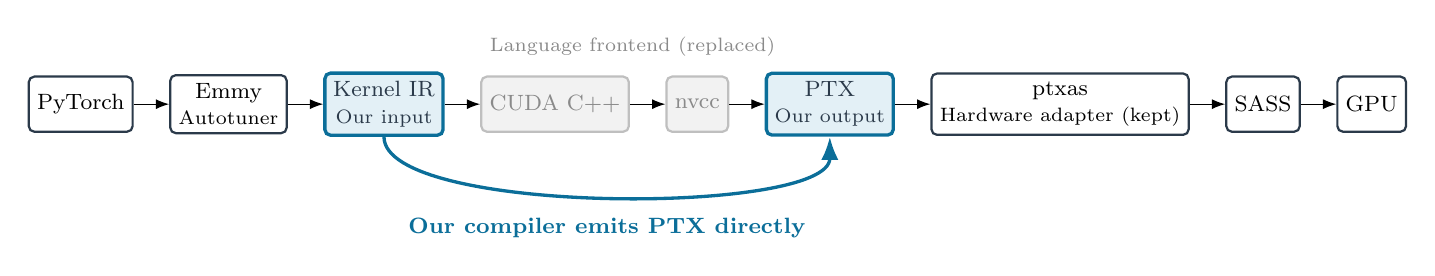
\begin{tikzpicture}[node distance=5mm and 4.5mm]
  \node[stage]                     (torch) {PyTorch};
  \node[stage,right=of torch]      (emmy)  {Emmy\\ \scriptsize Autotuner};
  \node[keystage,right=of emmy]    (ir)    {Kernel IR\\ \scriptsize Our input};
  \node[dimstage,right=of ir]      (cuda)  {CUDA C++};
  \node[dimstage,right=of cuda]    (nvcc)  {nvcc};
  \node[keystage,right=of nvcc]    (ptx)   {PTX\\ \scriptsize Our output};
  \node[stage,right=of ptx]        (ptxas) {ptxas\\ \scriptsize Hardware adapter (kept)};
  \node[stage,right=of ptxas]      (sass)  {SASS};
  \node[stage,right=of sass]       (gpu)   {GPU};

  \draw[-{Latex}] (torch) -- (emmy);
  \draw[-{Latex}] (emmy) -- (ir);
  \draw[-{Latex}] (ir) -- (cuda);
  \draw[-{Latex}] (cuda) -- (nvcc);
  \draw[-{Latex}] (nvcc) -- (ptx);
  \draw[-{Latex}] (ptx) -- (ptxas);
  \draw[-{Latex}] (ptxas) -- (sass);
  \draw[-{Latex}] (sass) -- (gpu);

  \node[font=\scriptsize,text=dimtext,above=1.2mm of cuda.north west,anchor=south west]
    {Language frontend (replaced)};
  \draw[-{Latex},very thick,accent]
    (ir.south) .. controls +(0,-1.0) and +(0,-1.0) .. (ptx.south)
    node[pos=0.5,below=1.5mm,font=\footnotesize\bfseries,text=accent]
    {Our compiler emits PTX directly};
\end{tikzpicture}%
}
\end{center}

\vspace{3mm}
{\footnotesize
\begin{itemize}\setlength{\itemsep}{1.5pt}
\item The autotuner compiles thousands of variants per kernel, so the middle
  step's cost is paid thousands of times.
\item The IR arrives fully scheduled. A strict contract means even a lookup
  table can emit valid PTX.
\end{itemize}}
\end{frame}

% ============================================================
\begin{frame}{What we built}

\begin{center}
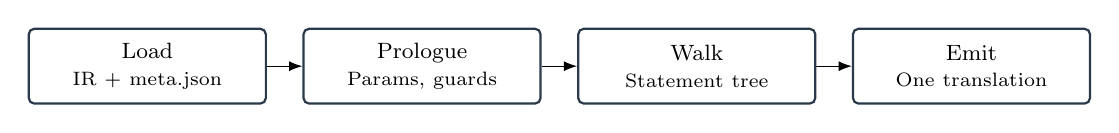
\begin{tikzpicture}[node distance=4.5mm,
  every node/.style={stage,minimum height=9.5mm,inner sep=3pt,text width=28mm}]
  \node (load) {Load\\ \scriptsize IR + meta.json};
  \node (pro)  [right=of load] {Prologue\\ \scriptsize Params, guards};
  \node (walk) [right=of pro]  {Walk\\ \scriptsize Statement tree};
  \node (emit) [right=of walk] {Emit\\ \scriptsize One translation};
  \draw[-{Latex}] (load) -- (pro);
  \draw[-{Latex}] (pro)  -- (walk);
  \draw[-{Latex}] (walk) -- (emit);
\end{tikzpicture}

\vspace{0.5mm}
{\scriptsize\color{dimtext} One kernel in, one PTX module out.}
\end{center}

\vspace{1.5mm}
\begin{center}
{\scriptsize
\begin{tabular}{@{}>{\raggedright\arraybackslash\color{ircol}\ttfamily}p{0.38\textwidth}@{}
                @{\hspace{7mm}}c
                >{\raggedright\arraybackslash\color{slate}\ttfamily}p{0.47\textwidth}@{}}
{\bfseries Kernel IR} & &
  {\bfseries Emitted PTX} \\[1.8mm]
arg\_order from meta.json & &
  .visible .entry k\_sum\_1\_reduce(\newline
  \hspace*{1.2em}.param .u64 param\_x,\newline
  \hspace*{1.2em}.param .u64 param\_sum\_1) \\[1.0mm]
in0 = load x[a0] & &
  ld.global.f32 \%f2, [\%rd6]; \\[1.0mm]
f32 acc0 <- add(acc0, in0) & &
  add.rn.f32 \%f1, \%f1, \%f2; \\[1.0mm]
WarpShuffle(acc0, length=32) & &
  shfl.sync.bfly.b32 \%r8, \%r7, 16, 0x1f, \%r6; \\
\end{tabular}}
\end{center}

\vspace{1.5mm}
{\scriptsize
\begin{itemize}\setlength{\itemsep}{1pt}
\item Fresh registers for every value, so a stale read cannot happen
\item Narrow types computed in f32, same as Emmy's own pipeline
\item Unsupported statements raise loudly instead of guessing
\end{itemize}}
\end{frame}

% ============================================================
\begin{frame}{Verification engine}

{\setlength{\tabcolsep}{3pt}
\begin{center}
{\renewcommand{\arraystretch}{1.15}\scriptsize
\begin{tabular}{@{}>{\raggedright\arraybackslash}m{25mm}
                >{\raggedright\arraybackslash\color{accent}}m{16.5mm}
                >{\raggedright\arraybackslash}m{25.5mm}
                >{\raggedright\arraybackslash}m{21mm}
                >{\raggedright\arraybackslash}m{23mm}
                >{\raggedright\arraybackslash}m{18.5mm}@{}}
{\bfseries\color{slate}Verifier} &
{\bfseries\color{slate}Approach} &
{\bfseries\color{slate}Goal} &
{\bfseries\color{slate}Can} &
{\bfseries\color{slate}Cannot} &
{\bfseries\color{slate}Caught} \\
\arrayrulecolor{gray!40}\midrule
{\bfseries\color{slate}Official runner} & Sampled &
  The exact judging pipeline & Anything breaking a real kernel &
  Ops the 15 problems never test & Inverted tanh, error 2.0 \\[0.5mm]
\arrayrulecolor{gray!22}\hline
{\bfseries\color{slate}ptxas sweep} & Exhaustive &
  Every op $\times$ dtype assembles & Invalid PTX, wrong types &
  Valid PTX, wrong math & mul.s32 is not an instruction \\[0.5mm]
\arrayrulecolor{gray!22}\hline
{\bfseries\color{slate}Semantic sweep} & Sampled &
  Every op $\times$ dtype vs numpy & Quietly wrong numbers &
  Ops interacting in one kernel & pow(-2,3) gave NaN, not -8 \\[0.5mm]
\arrayrulecolor{gray!22}\hline
{\bfseries\color{slate}Differential vs Emmy} & Sampled &
  Two compilers, same inputs & Divergence in output numbers &
  Shared misreadings & m02 reused one cached slab \\[0.5mm]
\arrayrulecolor{gray!22}\hline
{\bfseries\color{slate}Verification engine} & Proof-based &
  Proof conditions per compile & Broken SSA, stale caches &
  Wrong math in valid discipline & Nothing, 100 problems clean \\[0.5mm]
\arrayrulecolor{gray!22}\hline
{\bfseries\color{slate}Thread map proof} & Proof-based &
  Each thread maps to its cell & Wrong thread assignments &
  Runtime-only failures & a02 hit wrong cells before remap \\
\end{tabular}}
\end{center}}
\end{frame}

\end{document}
